\section{Frequenzanalyse}
\subsection{Fourier-Transformation}
\script{121} Um vom Zeitbereich in Frequenzbereich zu Transformieren mitt Funktion $f(t)$ mit der Fourier-Transformation integriert werden:
\[
	F(j\omega) = \int_{-\infty}^{\infty}f(t)e^{-j\omega t}dt
\]

Die Rücktransformation mit der inverse Fourier-Transformation:
\[
f(t) = \frac{1}{2\pi}\int_{-\infty}^{\infty}F(j\omega)e^{j\omega t}d\omega
\]

Die Konvergenzgeschwindigkeit kann im \script{123} nachgelesen werden.

\subsubsection{Eigenschaften}
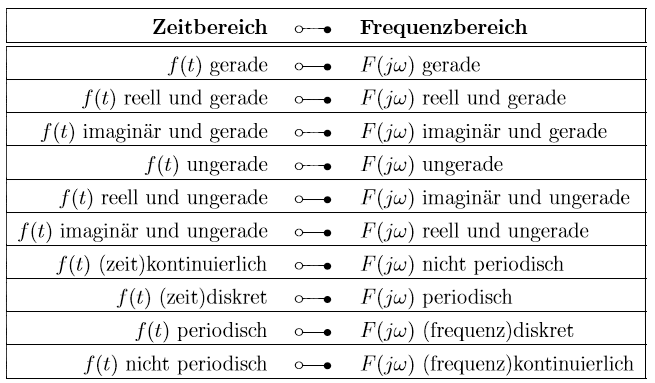
\includegraphics[width=\columnwidth]{Images/fourier_eigenschaten}
Weitere Eigenschaften sind im Skript auf Seite \script{124} zufinden.

\subsubsection{Symmetrie}
\textbf{ACHTUNG:} Gilt nur für $\mathbb{R}$ Fourierreihe! In $\mathbb{C}$ Reihe darf nicht über die halbe Periode Integriert und das Resultat verdoppelt werden! 
~\\
~\\
\noindent Für alle \textbf{geraden} (Achsensymmetrisch) T-periodische Funktionen ($f(t) = f(-t)$)  gilt $b_n = 0$ und für $a_n$ gilt:
\[
a_n = \frac{4}{T}\int_{0}^{\frac{T}{2}}f(t) \cdot \cos(n\omega t)dt
\]

\noindent Ist die Funktion \textbf{ungerade} (Punktsymmetrisch) ($f(-t) = -f(t)$) dann gilt $a_n = 0$ und für $b_n$:
\[
b_n = \frac{4}{T}\int_{0}^{\frac{T}{2}}f(t) \cdot \sin(n\omega t)dt 
\]


\subsubsection{Eigenschaften}
Einige wichtige Eigenschaften, weitere sind im \script{24}\\
\noindent\textbf{Funktionen}
\begin{align*}
	\delta(t) &\transform 1(\omega) \\
	u(t) &\transform \frac{1}{j\omega} \quad\text{(Einheitssprung)}\\
	\text{rect}_{-\frac{1}{2},\frac{1}{2}}(t) &\transform \sinc\left(\frac{\omega}{2}\right) \\
	\cos(\omega_0 t) &\transform \pi\left[\delta(\omega + \omega_0) + \delta(\omega - \omega_0)\right] \\
	\sin(\omega_0 t) &\transform j\pi\left[\delta(\omega + \omega_0) - \delta(\omega - \omega_0)\right]
\end{align*}

\noindent\textbf{Vertauschung}
\begin{align*}
	X(t) \transform 2\pi \cdot x(\-\omega)
\end{align*}

\noindent\textbf{Verschiebung im Zeitbereich}
\begin{align*}
	x(t - t_0) \transform X(\omega) \cdot e^{-j\omega t_0} 
\end{align*}

\noindent\textbf{Verschiebung im Frequenzbereich}
\begin{align*}
	x(t) \cdot e^{j\omega_0 t} \transform X(\omega - \omega_0)
\end{align*}

\noindent\textbf{Horizontale Streckung}
\begin{align*}
	x(\alpha \cdot t) \transform \frac{1}{|\alpha|}X\left(\frac{\omega}{\alpha}\right)
\end{align*}

\noindent\textbf{Modulationssatz}
\begin{align*}
	A_c \cdot x(t) \cdot \cos(\omega_0t) &\transform \frac{A_c}{2}\left[X(\omega - \omega_0) + X(\omega + \omega_0)\right] \\
	A_c \cdot x(t) \cdot \sin(\omega_0t) &\transform \frac{A_c}{2j}\left[X(\omega - \omega_0) - X(\omega + \omega_0)\right]
\end{align*}

\noindent\textbf{Differentation}
\begin{align*}
	\frac{dx}{dt}(t) \transform j\omega \cdot X(\omega)
\end{align*}

\noindent\textbf{Integration}
\begin{align*}
	\int_{-\infty}^{t}x(\tau)d\tau \transform X(\omega)\cdot \left(\frac{1}{j\omega} + \pi \delta(\omega)\right)
\end{align*}

\subsection{Laplace-Transformation}
\script{135} Die einseitige Laplace-Transformation transformiert die Zeitdomain in die s-Domain:
\[
F(s) = \int_{0}^{\infty}f(t)e^{-st}dt
\]

\subsubsection{Rücktransformation}
\script{140} Rücktransformation mit \textbf{gebrochen-rationaler Funktionen} ist via PBZ und dem Residuensatz oder mit Tabellen \script{159} zu berechnen:
\begin{align*}
	F(s) = \sum_{i=1}^{k}\sum_{j=1}^{n_k}\frac{A_{ij}}{(s-p_i)^j} \\
	f(t) = \left(\sum_{i=1}^{k}e^{p_it}\sum_{j=1}^{n_k}\frac{A_{ij}t^{j-1}}{(j-1)!}\right)u(t)
\end{align*}

Dabei können die Koeffizienten $A_{ij}$ berechnet werden mit dem Residuensatz:
\[
A_{ij} = \frac{1}{(n_i - j)!}\frac{\partial^{n_i-j}}{\partial s^{n_i -j}}[(s-{p_i})^{n_i}F(s)]|_{s_{p_i}}
\]

\subsubsection{Eigenschaften}
\script{136}


\subsection{DGL}
\textbf{Beispiel} $\ddot{u}(t) + \dot{u}(t) + u(t) = \sigma(t)\sin(2t)$ mit Anfang $u(0) = 0$ und $\dot{u}(0) = 0$
\[\dot{u}(t) \transform sU(s) - u(0+) \text{ und } \ddot{u}(t) \transform s^2U(s) - sU(0+) - \dot{u}(0+)\]
Dabei werden die Anfangswerte mit Limes identifizert zB: $u(0+) = \lim\limits_{t\rightarrow0+}u(t) = u(0) = 0$.
\[ \sigma(t)\sin(2t) = \frac{2}{s^2 + 2^2} \]
Nun wird die DGL in den Bildbereich transformiert.
\begin{align*}
	s^2U(s) + sU(s) + U(s) &= \frac{2}{s^2 + 2^2} \\
	U(s) &= \frac{2}{(s^2 + 4)(s^2 + s + 1)}
\end{align*}
Mittels PBZ kann dies wieder in den Zeitbereich transformiert werden.
\begin{align*}
	\frac{2}{(s^2 + 4)(s^2 + s + 1)} = \frac{as +b}{s^2 + 4}+\frac{cs + d}{s^2 + s + 1} \quad | \cdot HN \\
	2 = (a + c)s^3 + (a+b+d)s^2 + (a+b+4c)s + b + 4d
\end{align*}
Daraus lässt sich das LGS herleiten und die Parameter mit Koeffizientenvergleich bestimmen.
\[
\begin{matrix}
	a &  &   & + & c  &    &     & = 0 \\
	a &+ & b & + &    & +  & d   &= 0 \\
	a &+ & b & + & 4c &    &     & = 0 \\
	&  & b &   &    & +  & 4d  & = 2\\
\end{matrix} \qquad\xRightarrow[]{}\qquad
\begin{matrix}
	a &= \frac{-2}{13} \\
	b &=\frac{-6}{13} \\
	c &=\frac{2}{13} \\
	d &= \frac{8}{13}\\
\end{matrix}
\]
Zurück in den Zeitbereich transformieren mittels Umformungen (hier Quadratische Ergänzung $s^2 + s +1 = (s+\frac{1}{2})^2 + \frac{3}{4}$) und Laplace-Tabelle.
\begin{align*}
	U(s) =& -\frac{2}{13}\cdot\overbrace{\frac{s}{s^2 +2^2}}^{\cos(2t)} -\frac{2}{13}\cdot\frac{3}{2}\cdot\overbrace{\frac{2}{s^2 + 2^2}}^{\sin(2t)} \\
	& + \frac{2}{13}\cdot\underbrace{\frac{s + \frac{1}{2}}{(s+\frac{1}{2})^2 + \frac{3}{4}}}_{\cos\left(\frac{\sqrt{3}}{2}t\right)e^{-\frac{t}{2}}} + \frac{2}{13}\cdot\frac{7\sqrt{3}}{3}\cdot\underbrace{\frac{\frac{\sqrt{3}}{2}}{(s+\frac{1}{2})^2 + \frac{3}{4}}}_{\sin\left(\frac{\sqrt{3}}{2}t\right)e^{-\frac{t}{2}}} \\
\end{align*}
\begin{align*}
	u(t) = \sigma(t)&\left(-\frac{2}{13}\cos(2t) -\frac{3}{13}\sin(2t)\right) \\
	+ \sigma(t)&\left( \frac{2}{13}\cos\left(\frac{\sqrt{3}}{2}t\right)e^{-\frac{t}{2}} + \frac{14\sqrt{3}}{39}\sin\left(\frac{\sqrt{3}}{2}t\right)e^{-\frac{t}{2}}\right)
\end{align*}
